% Options for packages loaded elsewhere
\PassOptionsToPackage{unicode}{hyperref}
\PassOptionsToPackage{hyphens}{url}
%
\documentclass[
]{article}
\usepackage{amsmath,amssymb}
\usepackage{iftex}
\ifPDFTeX
  \usepackage[T1]{fontenc}
  \usepackage[utf8]{inputenc}
  \usepackage{textcomp} % provide euro and other symbols
\else % if luatex or xetex
  \usepackage{unicode-math} % this also loads fontspec
  \defaultfontfeatures{Scale=MatchLowercase}
  \defaultfontfeatures[\rmfamily]{Ligatures=TeX,Scale=1}
\fi
\usepackage{lmodern}
\ifPDFTeX\else
  % xetex/luatex font selection
\fi
% Use upquote if available, for straight quotes in verbatim environments
\IfFileExists{upquote.sty}{\usepackage{upquote}}{}
\IfFileExists{microtype.sty}{% use microtype if available
  \usepackage[]{microtype}
  \UseMicrotypeSet[protrusion]{basicmath} % disable protrusion for tt fonts
}{}
\makeatletter
\@ifundefined{KOMAClassName}{% if non-KOMA class
  \IfFileExists{parskip.sty}{%
    \usepackage{parskip}
  }{% else
    \setlength{\parindent}{0pt}
    \setlength{\parskip}{6pt plus 2pt minus 1pt}}
}{% if KOMA class
  \KOMAoptions{parskip=half}}
\makeatother
\usepackage{xcolor}
\usepackage[margin=1in]{geometry}
\usepackage{color}
\usepackage{fancyvrb}
\newcommand{\VerbBar}{|}
\newcommand{\VERB}{\Verb[commandchars=\\\{\}]}
\DefineVerbatimEnvironment{Highlighting}{Verbatim}{commandchars=\\\{\}}
% Add ',fontsize=\small' for more characters per line
\usepackage{framed}
\definecolor{shadecolor}{RGB}{248,248,248}
\newenvironment{Shaded}{\begin{snugshade}}{\end{snugshade}}
\newcommand{\AlertTok}[1]{\textcolor[rgb]{0.94,0.16,0.16}{#1}}
\newcommand{\AnnotationTok}[1]{\textcolor[rgb]{0.56,0.35,0.01}{\textbf{\textit{#1}}}}
\newcommand{\AttributeTok}[1]{\textcolor[rgb]{0.13,0.29,0.53}{#1}}
\newcommand{\BaseNTok}[1]{\textcolor[rgb]{0.00,0.00,0.81}{#1}}
\newcommand{\BuiltInTok}[1]{#1}
\newcommand{\CharTok}[1]{\textcolor[rgb]{0.31,0.60,0.02}{#1}}
\newcommand{\CommentTok}[1]{\textcolor[rgb]{0.56,0.35,0.01}{\textit{#1}}}
\newcommand{\CommentVarTok}[1]{\textcolor[rgb]{0.56,0.35,0.01}{\textbf{\textit{#1}}}}
\newcommand{\ConstantTok}[1]{\textcolor[rgb]{0.56,0.35,0.01}{#1}}
\newcommand{\ControlFlowTok}[1]{\textcolor[rgb]{0.13,0.29,0.53}{\textbf{#1}}}
\newcommand{\DataTypeTok}[1]{\textcolor[rgb]{0.13,0.29,0.53}{#1}}
\newcommand{\DecValTok}[1]{\textcolor[rgb]{0.00,0.00,0.81}{#1}}
\newcommand{\DocumentationTok}[1]{\textcolor[rgb]{0.56,0.35,0.01}{\textbf{\textit{#1}}}}
\newcommand{\ErrorTok}[1]{\textcolor[rgb]{0.64,0.00,0.00}{\textbf{#1}}}
\newcommand{\ExtensionTok}[1]{#1}
\newcommand{\FloatTok}[1]{\textcolor[rgb]{0.00,0.00,0.81}{#1}}
\newcommand{\FunctionTok}[1]{\textcolor[rgb]{0.13,0.29,0.53}{\textbf{#1}}}
\newcommand{\ImportTok}[1]{#1}
\newcommand{\InformationTok}[1]{\textcolor[rgb]{0.56,0.35,0.01}{\textbf{\textit{#1}}}}
\newcommand{\KeywordTok}[1]{\textcolor[rgb]{0.13,0.29,0.53}{\textbf{#1}}}
\newcommand{\NormalTok}[1]{#1}
\newcommand{\OperatorTok}[1]{\textcolor[rgb]{0.81,0.36,0.00}{\textbf{#1}}}
\newcommand{\OtherTok}[1]{\textcolor[rgb]{0.56,0.35,0.01}{#1}}
\newcommand{\PreprocessorTok}[1]{\textcolor[rgb]{0.56,0.35,0.01}{\textit{#1}}}
\newcommand{\RegionMarkerTok}[1]{#1}
\newcommand{\SpecialCharTok}[1]{\textcolor[rgb]{0.81,0.36,0.00}{\textbf{#1}}}
\newcommand{\SpecialStringTok}[1]{\textcolor[rgb]{0.31,0.60,0.02}{#1}}
\newcommand{\StringTok}[1]{\textcolor[rgb]{0.31,0.60,0.02}{#1}}
\newcommand{\VariableTok}[1]{\textcolor[rgb]{0.00,0.00,0.00}{#1}}
\newcommand{\VerbatimStringTok}[1]{\textcolor[rgb]{0.31,0.60,0.02}{#1}}
\newcommand{\WarningTok}[1]{\textcolor[rgb]{0.56,0.35,0.01}{\textbf{\textit{#1}}}}
\usepackage{graphicx}
\makeatletter
\def\maxwidth{\ifdim\Gin@nat@width>\linewidth\linewidth\else\Gin@nat@width\fi}
\def\maxheight{\ifdim\Gin@nat@height>\textheight\textheight\else\Gin@nat@height\fi}
\makeatother
% Scale images if necessary, so that they will not overflow the page
% margins by default, and it is still possible to overwrite the defaults
% using explicit options in \includegraphics[width, height, ...]{}
\setkeys{Gin}{width=\maxwidth,height=\maxheight,keepaspectratio}
% Set default figure placement to htbp
\makeatletter
\def\fps@figure{htbp}
\makeatother
\setlength{\emergencystretch}{3em} % prevent overfull lines
\providecommand{\tightlist}{%
  \setlength{\itemsep}{0pt}\setlength{\parskip}{0pt}}
\setcounter{secnumdepth}{-\maxdimen} % remove section numbering
\usepackage{fvextra}
\DefineVerbatimEnvironment{Highlighting}{Verbatim}{breaklines,commandchars=\\\{\}}
\ifLuaTeX
  \usepackage{selnolig}  % disable illegal ligatures
\fi
\usepackage{bookmark}
\IfFileExists{xurl.sty}{\usepackage{xurl}}{} % add URL line breaks if available
\urlstyle{same}
\hypersetup{
  pdftitle={SDA Group Submission Assignment Assign5},
  pdfauthor={MengliFeng (2720589) and PepijnVanOostveen (2801582)},
  hidelinks,
  pdfcreator={LaTeX via pandoc}}

\title{SDA Group Submission Assignment Assign5}
\usepackage{etoolbox}
\makeatletter
\providecommand{\subtitle}[1]{% add subtitle to \maketitle
  \apptocmd{\@title}{\par {\large #1 \par}}{}{}
}
\makeatother
\subtitle{Group Gr18}
\author{MengliFeng (2720589) and PepijnVanOostveen (2801582)}
\date{}

\begin{document}
\maketitle

\section{Exercise 1}\label{exercise-1}

\begin{Shaded}
\begin{Highlighting}[]
\CommentTok{\# Load the data}
\NormalTok{grades }\OtherTok{\textless{}{-}} \FunctionTok{readRDS}\NormalTok{(}\StringTok{"grades.RDS"}\NormalTok{)}
\NormalTok{on\_time }\OtherTok{\textless{}{-}}\NormalTok{ grades}\SpecialCharTok{$}\NormalTok{on\_time}
\NormalTok{late }\OtherTok{\textless{}{-}}\NormalTok{ grades}\SpecialCharTok{$}\NormalTok{late}
\end{Highlighting}
\end{Shaded}

\subsection{a.}\label{a.}

\begin{Shaded}
\begin{Highlighting}[]
\CommentTok{\# Shapiro{-}Wilk Test for normality}
\NormalTok{shapiro\_on\_time }\OtherTok{\textless{}{-}} \FunctionTok{shapiro.test}\NormalTok{(on\_time)}
\NormalTok{shapiro\_late }\OtherTok{\textless{}{-}} \FunctionTok{shapiro.test}\NormalTok{(late)}

\CommentTok{\# Print results}
\FunctionTok{cat}\NormalTok{(}\StringTok{"Shapiro{-}Wilk Test for on\_time:}\SpecialCharTok{\textbackslash{}n}\StringTok{"}\NormalTok{)}
\end{Highlighting}
\end{Shaded}

\begin{verbatim}
## Shapiro-Wilk Test for on_time:
\end{verbatim}

\begin{Shaded}
\begin{Highlighting}[]
\FunctionTok{print}\NormalTok{(shapiro\_on\_time)}
\end{Highlighting}
\end{Shaded}

\begin{verbatim}
## 
##  Shapiro-Wilk normality test
## 
## data:  on_time
## W = 0.86829, p-value = 7.731e-14
\end{verbatim}

\begin{Shaded}
\begin{Highlighting}[]
\FunctionTok{cat}\NormalTok{(}\StringTok{"}\SpecialCharTok{\textbackslash{}n}\StringTok{Shapiro{-}Wilk Test for late:}\SpecialCharTok{\textbackslash{}n}\StringTok{"}\NormalTok{)}
\end{Highlighting}
\end{Shaded}

\begin{verbatim}
## 
## Shapiro-Wilk Test for late:
\end{verbatim}

\begin{Shaded}
\begin{Highlighting}[]
\FunctionTok{print}\NormalTok{(shapiro\_late)}
\end{Highlighting}
\end{Shaded}

\begin{verbatim}
## 
##  Shapiro-Wilk normality test
## 
## data:  late
## W = 0.87859, p-value = 0.006463
\end{verbatim}

for the on-time sample, the null hypothesis is rejected for the late
sample, the null hypothesis is rejected Since the null hypothesis for
Shapiro-Wilk test is that the data is normally distributed and it is
rejected for both of the samples, we know that t-test (requires normal
distribution of the samples) is not an approriate location test for the
data

\subsection{b.}\label{b.}

\begin{Shaded}
\begin{Highlighting}[]
\CommentTok{\# Remove values equal to 7, as they don\textquotesingle{}t contribute to the sign test}
\NormalTok{filtered\_on\_time }\OtherTok{\textless{}{-}}\NormalTok{ on\_time[on\_time }\SpecialCharTok{!=} \DecValTok{7}\NormalTok{]}

\CommentTok{\# Count how many are greater than 7}
\NormalTok{n }\OtherTok{\textless{}{-}} \FunctionTok{length}\NormalTok{(filtered\_on\_time)}
\NormalTok{num\_positive }\OtherTok{\textless{}{-}} \FunctionTok{sum}\NormalTok{(filtered\_on\_time }\SpecialCharTok{\textgreater{}} \DecValTok{7}\NormalTok{)}

\CommentTok{\# Exact binomial test (sign test)}
\NormalTok{sign\_test }\OtherTok{\textless{}{-}} \FunctionTok{binom.test}\NormalTok{(num\_positive, n, }\AttributeTok{p =} \FloatTok{0.5}\NormalTok{, }\AttributeTok{alternative =} \StringTok{"greater"}\NormalTok{)}
\FunctionTok{cat}\NormalTok{(}\StringTok{"}\SpecialCharTok{\textbackslash{}n}\StringTok{Sign Test Result (on\_time \textgreater{} 7):}\SpecialCharTok{\textbackslash{}n}\StringTok{"}\NormalTok{)}
\end{Highlighting}
\end{Shaded}

\begin{verbatim}
## 
## Sign Test Result (on_time > 7):
\end{verbatim}

\begin{Shaded}
\begin{Highlighting}[]
\FunctionTok{print}\NormalTok{(sign\_test)}
\end{Highlighting}
\end{Shaded}

\begin{verbatim}
## 
##  Exact binomial test
## 
## data:  num_positive and n
## number of successes = 170, number of trials = 250, p-value = 6.38e-09
## alternative hypothesis: true probability of success is greater than 0.5
## 95 percent confidence interval:
##  0.6280437 1.0000000
## sample estimates:
## probability of success 
##                   0.68
\end{verbatim}

\begin{Shaded}
\begin{Highlighting}[]
\CommentTok{\# Normal approximation}
\CommentTok{\# Mean and standard deviation under H0}
\NormalTok{mu }\OtherTok{\textless{}{-}}\NormalTok{ n }\SpecialCharTok{*} \FloatTok{0.5}
\NormalTok{sigma }\OtherTok{\textless{}{-}} \FunctionTok{sqrt}\NormalTok{(n }\SpecialCharTok{*} \FloatTok{0.5} \SpecialCharTok{*} \FloatTok{0.5}\NormalTok{)}

\CommentTok{\# Normal approximation (continuity correction)}
\NormalTok{z }\OtherTok{\textless{}{-}}\NormalTok{ (num\_positive }\SpecialCharTok{{-}}\NormalTok{ mu ) }\SpecialCharTok{/}\NormalTok{ sigma}
\NormalTok{p\_norm }\OtherTok{\textless{}{-}} \DecValTok{1} \SpecialCharTok{{-}} \FunctionTok{pnorm}\NormalTok{(z)}
\FunctionTok{cat}\NormalTok{(}\StringTok{"}\SpecialCharTok{\textbackslash{}n}\StringTok{Normal approximation p{-}value:}\SpecialCharTok{\textbackslash{}n}\StringTok{"}\NormalTok{)}
\end{Highlighting}
\end{Shaded}

\begin{verbatim}
## 
## Normal approximation p-value:
\end{verbatim}

\begin{Shaded}
\begin{Highlighting}[]
\FunctionTok{print}\NormalTok{(p\_norm)}
\end{Highlighting}
\end{Shaded}

\begin{verbatim}
## [1] 6.274324e-09
\end{verbatim}

the null hypothesis under the sign test is rejected the p-value for the
normal approximation is slightly larger than that under sign test, with
magnitude of e-9. the null hypothesis for the normal approximation is
also rejected.

\subsection{c.}\label{c.}

\begin{Shaded}
\begin{Highlighting}[]
\CommentTok{\# Remove values equal to 7}
\NormalTok{filtered\_late }\OtherTok{\textless{}{-}}\NormalTok{ late[late }\SpecialCharTok{!=} \DecValTok{7}\NormalTok{]}

\CommentTok{\# Count how many are greater than 7}
\NormalTok{n\_late }\OtherTok{\textless{}{-}} \FunctionTok{length}\NormalTok{(filtered\_late)}
\NormalTok{num\_positive\_late }\OtherTok{\textless{}{-}} \FunctionTok{sum}\NormalTok{(filtered\_late }\SpecialCharTok{\textgreater{}} \DecValTok{7}\NormalTok{)}

\CommentTok{\# Exact binomial test (sign test)}
\NormalTok{sign\_test\_late }\OtherTok{\textless{}{-}} \FunctionTok{binom.test}\NormalTok{(num\_positive\_late, n\_late, }\AttributeTok{p =} \FloatTok{0.5}\NormalTok{, }\AttributeTok{alternative =} \StringTok{"greater"}\NormalTok{)}
\FunctionTok{cat}\NormalTok{(}\StringTok{"}\SpecialCharTok{\textbackslash{}n}\StringTok{Sign Test Result (late \textgreater{} 7):}\SpecialCharTok{\textbackslash{}n}\StringTok{"}\NormalTok{)}
\end{Highlighting}
\end{Shaded}

\begin{verbatim}
## 
## Sign Test Result (late > 7):
\end{verbatim}

\begin{Shaded}
\begin{Highlighting}[]
\FunctionTok{print}\NormalTok{(sign\_test\_late)}
\end{Highlighting}
\end{Shaded}

\begin{verbatim}
## 
##  Exact binomial test
## 
## data:  num_positive_late and n_late
## number of successes = 17, number of trials = 25, p-value = 0.05388
## alternative hypothesis: true probability of success is greater than 0.5
## 95 percent confidence interval:
##  0.4963584 1.0000000
## sample estimates:
## probability of success 
##                   0.68
\end{verbatim}

\begin{Shaded}
\begin{Highlighting}[]
\CommentTok{\# Normal approximation}
\NormalTok{mu\_late }\OtherTok{\textless{}{-}}\NormalTok{ n\_late }\SpecialCharTok{*} \FloatTok{0.5}
\NormalTok{sigma\_late }\OtherTok{\textless{}{-}} \FunctionTok{sqrt}\NormalTok{(n\_late }\SpecialCharTok{*} \FloatTok{0.5} \SpecialCharTok{*} \FloatTok{0.5}\NormalTok{)}
\NormalTok{z\_late }\OtherTok{\textless{}{-}}\NormalTok{ (num\_positive\_late }\SpecialCharTok{{-}}\NormalTok{ mu\_late) }\SpecialCharTok{/}\NormalTok{ sigma\_late}
\NormalTok{p\_norm\_late }\OtherTok{\textless{}{-}} \DecValTok{1} \SpecialCharTok{{-}} \FunctionTok{pnorm}\NormalTok{(z\_late)}
\FunctionTok{cat}\NormalTok{(}\StringTok{"}\SpecialCharTok{\textbackslash{}n}\StringTok{Normal approximation p{-}value (late):}\SpecialCharTok{\textbackslash{}n}\StringTok{"}\NormalTok{)}
\end{Highlighting}
\end{Shaded}

\begin{verbatim}
## 
## Normal approximation p-value (late):
\end{verbatim}

\begin{Shaded}
\begin{Highlighting}[]
\FunctionTok{print}\NormalTok{(p\_norm\_late)}
\end{Highlighting}
\end{Shaded}

\begin{verbatim}
## [1] 0.03593032
\end{verbatim}

the normal approximation also lead to rejection of null hypothesis as
the sign test does, but the p-value is off for around 0.0179. The reason
is that binomial can be approximated by normal distribution with large
sample size. As \(n = 25\) (small sample size) and \(p = 0.5\),
\(n \cdot p \cdot(1-p) < 10\), the p-valule from normal distribution is
less accurate.

\section{Exercise 2}\label{exercise-2}

\subsection{a.}\label{a.-1}

\begin{Shaded}
\begin{Highlighting}[]
\CommentTok{\# load the samples and split it into the first 20 observations and the rest.}
\NormalTok{samples }\OtherTok{\textless{}{-}} \FunctionTok{readRDS}\NormalTok{(}\StringTok{"newcomb.RDS"}\NormalTok{)}
\NormalTok{sample1 }\OtherTok{\textless{}{-}}\NormalTok{ samples[}\DecValTok{1}\SpecialCharTok{:}\DecValTok{20}\NormalTok{]}
\NormalTok{sample2 }\OtherTok{\textless{}{-}}\NormalTok{ samples[}\DecValTok{21}\SpecialCharTok{:}\DecValTok{66}\NormalTok{]}

\CommentTok{\# set up plot layout. Two columns for the 2 sets of data and 3 rows for the 3 different plots}
\FunctionTok{par}\NormalTok{(}\AttributeTok{mfrow =} \FunctionTok{c}\NormalTok{(}\DecValTok{1}\NormalTok{, }\DecValTok{3}\NormalTok{))}

\CommentTok{\# histogram}
\NormalTok{breaks }\OtherTok{\textless{}{-}} \FunctionTok{pretty}\NormalTok{(}\FunctionTok{range}\NormalTok{(samples), }\AttributeTok{n =} \DecValTok{20}\NormalTok{)}

\FunctionTok{hist}\NormalTok{(sample2, }\AttributeTok{freq =} \ConstantTok{FALSE}\NormalTok{, }\AttributeTok{breaks=}\NormalTok{breaks, }\AttributeTok{col =} \FunctionTok{rgb}\NormalTok{(}\DecValTok{0}\NormalTok{, }\DecValTok{1}\NormalTok{, }\DecValTok{0}\NormalTok{, }\DecValTok{1}\SpecialCharTok{/}\DecValTok{4}\NormalTok{), }\AttributeTok{xlim =} \FunctionTok{range}\NormalTok{(samples),}
     \AttributeTok{main =} \StringTok{"Overlayed Histograms"}\NormalTok{, }\AttributeTok{xlab =} \StringTok{"Value"}\NormalTok{)}
\FunctionTok{hist}\NormalTok{(sample1, }\AttributeTok{freq =} \ConstantTok{FALSE}\NormalTok{, }\AttributeTok{breaks=}\NormalTok{breaks, }\AttributeTok{col =} \FunctionTok{rgb}\NormalTok{(}\DecValTok{0}\NormalTok{, }\DecValTok{0}\NormalTok{, }\DecValTok{1}\NormalTok{, }\DecValTok{1}\SpecialCharTok{/}\DecValTok{4}\NormalTok{),}\AttributeTok{xlim =} \FunctionTok{range}\NormalTok{(samples), }\AttributeTok{add =} \ConstantTok{TRUE}\NormalTok{)}
\FunctionTok{legend}\NormalTok{(}\StringTok{"topleft"}\NormalTok{, }\AttributeTok{legend =} \FunctionTok{c}\NormalTok{(}\StringTok{"Sample 1"}\NormalTok{, }\StringTok{"Sample 2"}\NormalTok{),}
       \AttributeTok{fill =} \FunctionTok{c}\NormalTok{(}\FunctionTok{rgb}\NormalTok{(}\DecValTok{0}\NormalTok{, }\DecValTok{0}\NormalTok{, }\DecValTok{1}\NormalTok{, }\DecValTok{1}\SpecialCharTok{/}\DecValTok{4}\NormalTok{), }\FunctionTok{rgb}\NormalTok{(}\DecValTok{0}\NormalTok{, }\DecValTok{1}\NormalTok{, }\DecValTok{0}\NormalTok{, }\DecValTok{1}\SpecialCharTok{/}\DecValTok{4}\NormalTok{)))}


\CommentTok{\# Boxplot}
\FunctionTok{boxplot}\NormalTok{(sample1, sample2, }\AttributeTok{names =} \FunctionTok{c}\NormalTok{(}\StringTok{"Sample 1"}\NormalTok{, }\StringTok{"Sample 2"}\NormalTok{), }\AttributeTok{col =} \FunctionTok{c}\NormalTok{(}\FunctionTok{rgb}\NormalTok{(}\DecValTok{0}\NormalTok{, }\DecValTok{0}\NormalTok{, }\DecValTok{1}\NormalTok{, }\DecValTok{1}\SpecialCharTok{/}\DecValTok{4}\NormalTok{), }\FunctionTok{rgb}\NormalTok{(}\DecValTok{0}\NormalTok{, }\DecValTok{1}\NormalTok{, }\DecValTok{0}\NormalTok{,  }\DecValTok{1}\SpecialCharTok{/}\DecValTok{4}\NormalTok{)),}
        \AttributeTok{main =} \StringTok{"Boxplots of both samples"}\NormalTok{, }\AttributeTok{ylab =} \StringTok{"Value"}\NormalTok{)}


\CommentTok{\# empirical CDF}
\FunctionTok{plot}\NormalTok{(}\FunctionTok{ecdf}\NormalTok{(sample1), }\AttributeTok{verticals =} \ConstantTok{TRUE}\NormalTok{, }\AttributeTok{do.points =} \ConstantTok{FALSE}\NormalTok{, }\AttributeTok{col =} \FunctionTok{rgb}\NormalTok{(}\DecValTok{0}\NormalTok{, }\DecValTok{0}\NormalTok{, }\DecValTok{1}\NormalTok{, }\DecValTok{1}\SpecialCharTok{/}\DecValTok{2}\NormalTok{),}
     \AttributeTok{main =} \StringTok{"ECDFs of Sample 1 and 2"}\NormalTok{, }\AttributeTok{xlab =} \StringTok{"Value"}\NormalTok{, }\AttributeTok{ylab =} \StringTok{"ECDF"}\NormalTok{)}
\FunctionTok{lines}\NormalTok{(}\FunctionTok{ecdf}\NormalTok{(sample2), }\AttributeTok{verticals =} \ConstantTok{TRUE}\NormalTok{, }\AttributeTok{do.points =} \ConstantTok{FALSE}\NormalTok{, }\AttributeTok{col =} \FunctionTok{rgb}\NormalTok{(}\DecValTok{0}\NormalTok{, }\DecValTok{1}\NormalTok{, }\DecValTok{0}\NormalTok{, }\DecValTok{1}\SpecialCharTok{/}\DecValTok{2}\NormalTok{))}
\FunctionTok{legend}\NormalTok{(}\StringTok{"topleft"}\NormalTok{, }\AttributeTok{legend =} \FunctionTok{c}\NormalTok{(}\StringTok{"Sample 1"}\NormalTok{, }\StringTok{"Sample 2"}\NormalTok{), }\AttributeTok{col =} \FunctionTok{c}\NormalTok{(}\FunctionTok{rgb}\NormalTok{(}\DecValTok{0}\NormalTok{, }\DecValTok{0}\NormalTok{, }\DecValTok{1}\NormalTok{,  }\DecValTok{1}\SpecialCharTok{/}\DecValTok{2}\NormalTok{), }\FunctionTok{rgb}\NormalTok{(}\DecValTok{0}\NormalTok{, }\DecValTok{1}\NormalTok{, }\DecValTok{0}\NormalTok{,  }\DecValTok{1}\SpecialCharTok{/}\DecValTok{2}\NormalTok{)), }\AttributeTok{lty =} \DecValTok{1}\NormalTok{)}
\end{Highlighting}
\end{Shaded}

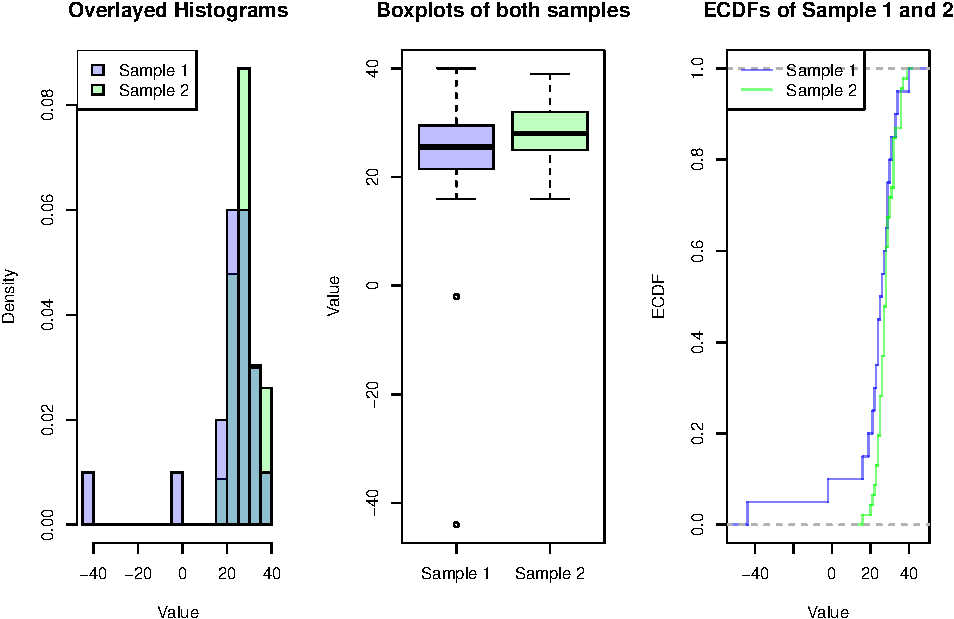
\includegraphics{SDA_submission_template_files/figure-latex/unnamed-chunk-5-1.pdf}
Sample 2 looks like it could be the result of a normal distribution and
the first 20 observations (sample 1) would also look like it comes from
a normal distribution, but only if the 2 outliers were removed. These
two outliers from sample 1 are the only outliers and make sample 1
asymmetric, while sample 2 isn't completely symmetric but is close to
it. (I used rgb values as colors since I needed transparent colors for
the histogram and wanted to use the same colors in the other graphs. I
reduced the transparency in the ECDF for better visibility.)

\begin{Shaded}
\begin{Highlighting}[]
\NormalTok{sample1\_trimmed }\OtherTok{\textless{}{-}} \FunctionTok{sort}\NormalTok{(sample1)[}\SpecialCharTok{{-}}\FunctionTok{c}\NormalTok{(}\DecValTok{1}\NormalTok{, }\DecValTok{2}\NormalTok{)]}
\FunctionTok{hist}\NormalTok{(sample1\_trimmed, }\AttributeTok{freq =} \ConstantTok{FALSE}\NormalTok{, }\AttributeTok{col =} \FunctionTok{rgb}\NormalTok{(}\DecValTok{0}\NormalTok{, }\DecValTok{0}\NormalTok{, }\DecValTok{1}\NormalTok{, }\DecValTok{1}\SpecialCharTok{/}\DecValTok{2}\NormalTok{),}
     \AttributeTok{main =} \StringTok{"Histogram of Sample 1 (2 lowest values removed)"}\NormalTok{, }\AttributeTok{xlab =} \StringTok{"Value"}\NormalTok{)}
\end{Highlighting}
\end{Shaded}

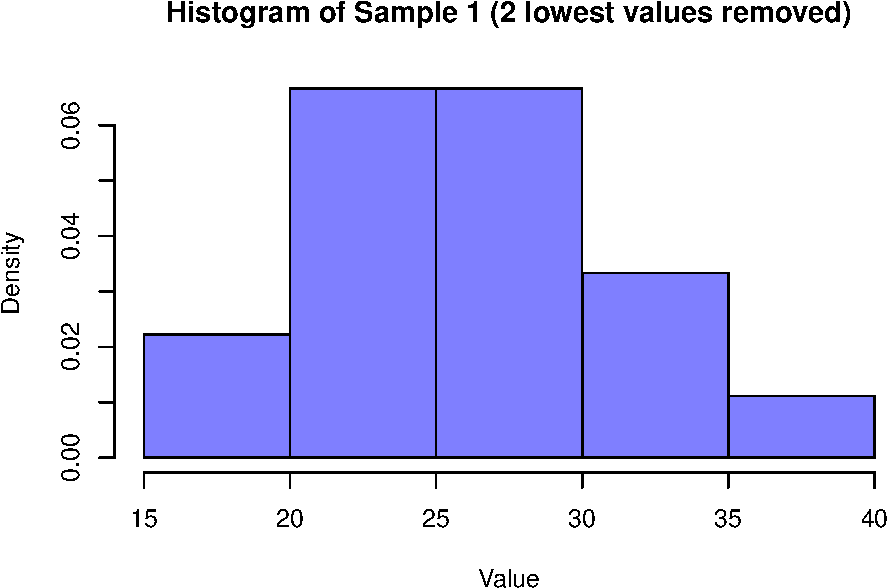
\includegraphics{SDA_submission_template_files/figure-latex/unnamed-chunk-6-1.pdf}
This histogram shows that the first 20 observations do indeed resemble a
normal distribution if the outliers are removed.

\subsection{b.}\label{b.-1}

The Wilcoxon two-sample test assumes that the distributions are the same
shape and looks at the location of these shapes. This is probably a bad
test for our sampels due to the outliers and we don't know if both
samples come from a normal distribution.' So the Kolmogorov-Smirnov
two-sample test is probably the best test since it tests if the samples
come from the same distribution shape.

\subsection{c.}\label{c.-1}

\begin{Shaded}
\begin{Highlighting}[]
\NormalTok{ks\_result }\OtherTok{\textless{}{-}} \FunctionTok{ks.test}\NormalTok{(sample1, sample2)}
\NormalTok{ks\_result}
\end{Highlighting}
\end{Shaded}

\begin{verbatim}
## 
##  Exact two-sample Kolmogorov-Smirnov test
## 
## data:  sample1 and sample2
## D = 0.25435, p-value = 0.1776
## alternative hypothesis: two-sided
\end{verbatim}

The p-value is higher than our significance level of 0.05 and thus we
don't reject our hypothesis that the two distributions come from the
same distribution. With how low the p-value is I would say that we don't
know if the two samples come from the same distribution without context.

With context I would say that a reasonable explanation for the
difference is that the error of experiment is normally distributed and
that the Newcomb became better at the experiment as he went along so the
only 2 outliers happened in the first 20 observations. Let us remove
this two possible mistakes and do the test again.

\begin{Shaded}
\begin{Highlighting}[]
\NormalTok{ks\_result }\OtherTok{\textless{}{-}} \FunctionTok{ks.test}\NormalTok{(sample1\_trimmed, sample2)}
\NormalTok{ks\_result}
\end{Highlighting}
\end{Shaded}

\begin{verbatim}
## 
##  Exact two-sample Kolmogorov-Smirnov test
## 
## data:  sample1_trimmed and sample2
## D = 0.19324, p-value = 0.4917
## alternative hypothesis: two-sided
\end{verbatim}

The p-value is 0.4917 and my conclusion is that we still can't be very
confident one way or another.

\end{document}
